\section{Results \& Discussion}

\subsection{Be}
\begin{table}
    \begin{threeparttable}
    \caption{\label{tab:wfn_BE} PAs of \ce{Be} calculated using various methods. The methods and basis used as reported as "without $e^{+}$ method or basis // with $e^{+}$ method or basis". We also report if the $s^2 \rightarrow p^2$ near degeneracy is handled.}
    \begin{tabular}{lrl}
method                          & PA (meV)    & $s^2 \rightarrow p^2$ \\ \hline
HF // HF    \tnote{1}           & -1.9        & no  \\
HF // rSDCI \tnote{1}           & 152.3       & no  \\
FCI // FCI  \tnote{1}           & 10.5        & yes \\ \hline

DMC\cite{10.1063/1.1486447}              & 100 $\pm$ 5 & no  \\
DMC\cite{10.1063/1.1486447}              & 33 $\pm$ 11 & yes \\
SVM\cite{10.4208/jams.071510.072110a}    & 86          & yes \\
DMC\cite{10.1021/acs.jctc.1c01193}       & 34 $\pm$ 8  & yes \\
DMC\cite{10.1021/acs.jctc.1c01193}       & 54 $\pm$ 10 & yes \\
\end{tabular}
\begin{tablenotes}
  \item [1] These calculations used the aug-cc-pVQZ basis set for the electrons and an 11s8p6d6f3g basis for the positron.
\end{tablenotes}
\end{threeparttable}
\end{table}

We first consider a positron binding to a \ce{Be} atom. 
%This system serves as a simple case where the positron is bound by correlation as the parent \ce{Be} atom is not charged.
Table~\ref{tab:wfn_BE} contains the positron affinity for \ce{Be} calculated with several methods.
Also tabulated are results from the literature using the \gls{dmc} and \gls{svm} methods.
As expected, the \gls{hf} treatment fails to bind the positron.
The \gls{rSDCI} approach, which includes all single excitations and only the double excitations that involve the positron, greatly increases the binding energy, in fact giving a value about 60\% too large in magnitude.
%This is attributed to the incorporation \ce{e-}/\ce{e+} dispersion missing in the \glsxtrlong{mf} treatment.
%We expect that higher order excitations which would capture orbital relaxation effects would decrease the positron affinity.
In the FCI results, the binding energy drops significantly.
This is both due to the inclusion of the higher order corrections to the dispersion, but also including the superposition of configurations from the $s^2 \rightarrow p^2$ near degeneracy.
Since this is calculated using a Gaussian basis, we expect that this is still not fully resolving the electron-positron cusp.

The DMC results for the positron affinity of \ce{Be} is presented in table~\ref{tab:DMC_BE}.
The positron affinities are presented for the zero time step extrapolated DMC energies with various trial wave functions.
Using the Jastrow factor with a multi-Slater determinant trial function explicitly includes the electron-positron cusp.
The three single determinant references yield similar \gls{pa}.
The single determinant energy versus time step for \ce{Be} with a positron is presented in figure~\ref{fig:be_sd_extrap}.
For each of the single determinant wave functions, the extrapolated \gls{dmc} energies are within error bars of each other.
The \gls{hf} nodal surface is expected to be the poorest as the positron is unbound in that case, which manifests as it has the largest time step dependence and the largest error bars in the same projection time.
These results also show that the $s^2 \rightarrow p^2$ near degeneracy cannot be captured by a single Slater determinant as the \gls{fci} wave function captures this effect, but the natural orbitals from the \gls{fci} wave function do not.

\begin{table}
    \caption{\label{tab:DMC_BE} PAs of \ce{Be} calculated using the DMC method and various trial wave functions. The trial wave functions used are reported as "single or multi- determinant/ without $e^{+}$ wfn // SD or MD / with $e^{+}$ wfn". }
    \begin{tabular}{lr}
trial wave function          &  PA (meV) \\ \hline
SD/HF//SD/HF                 &  96  $\pm$ 5 \\
SD/HF//SD/NO rSDCI           &  104 $\pm$ 4 \\
SD/FCI NO//SD/FCI NO         &  95  $\pm$ 4 \\ \hline
SD/HF//MD/rSDCI              &  151 $\pm$ 4 \\
MD/FCI   //MD/FCI            &  91 $\pm$  4 \\
\end{tabular}
\end{table}

The \gls{dmc} results from the literature, tabulated in table~\ref{tab:wfn_BE}, show the same marked decrease in the \gls{pa} by including the $s^2\rightarrow p^2$ excitations.
With a more sophisticated treatment of electron-positron correlation, the \gls{pa} nearly doubles as seen in table~\ref{tab:wfn_BE}.\cite{10.1021/acs.jctc.1c01193}
This indicates a strong impact of the correlation on the nodal surface.

\begin{figure}
    \caption{\label{fig:be_sd_extrap} The DMC energy versus time step for \ce{Be} with a bound positron using a trial wave function of a single determinant of Hartree-Fock orbitals, frozen core rSDCI natural orbitals, and frozen core FCI natural orbitals. The shading represents the error in the linear fit to the \gls{dmc} data. All plots generated using Matplotlib.\cite{10.1109/MCSE.2007.55}}.
    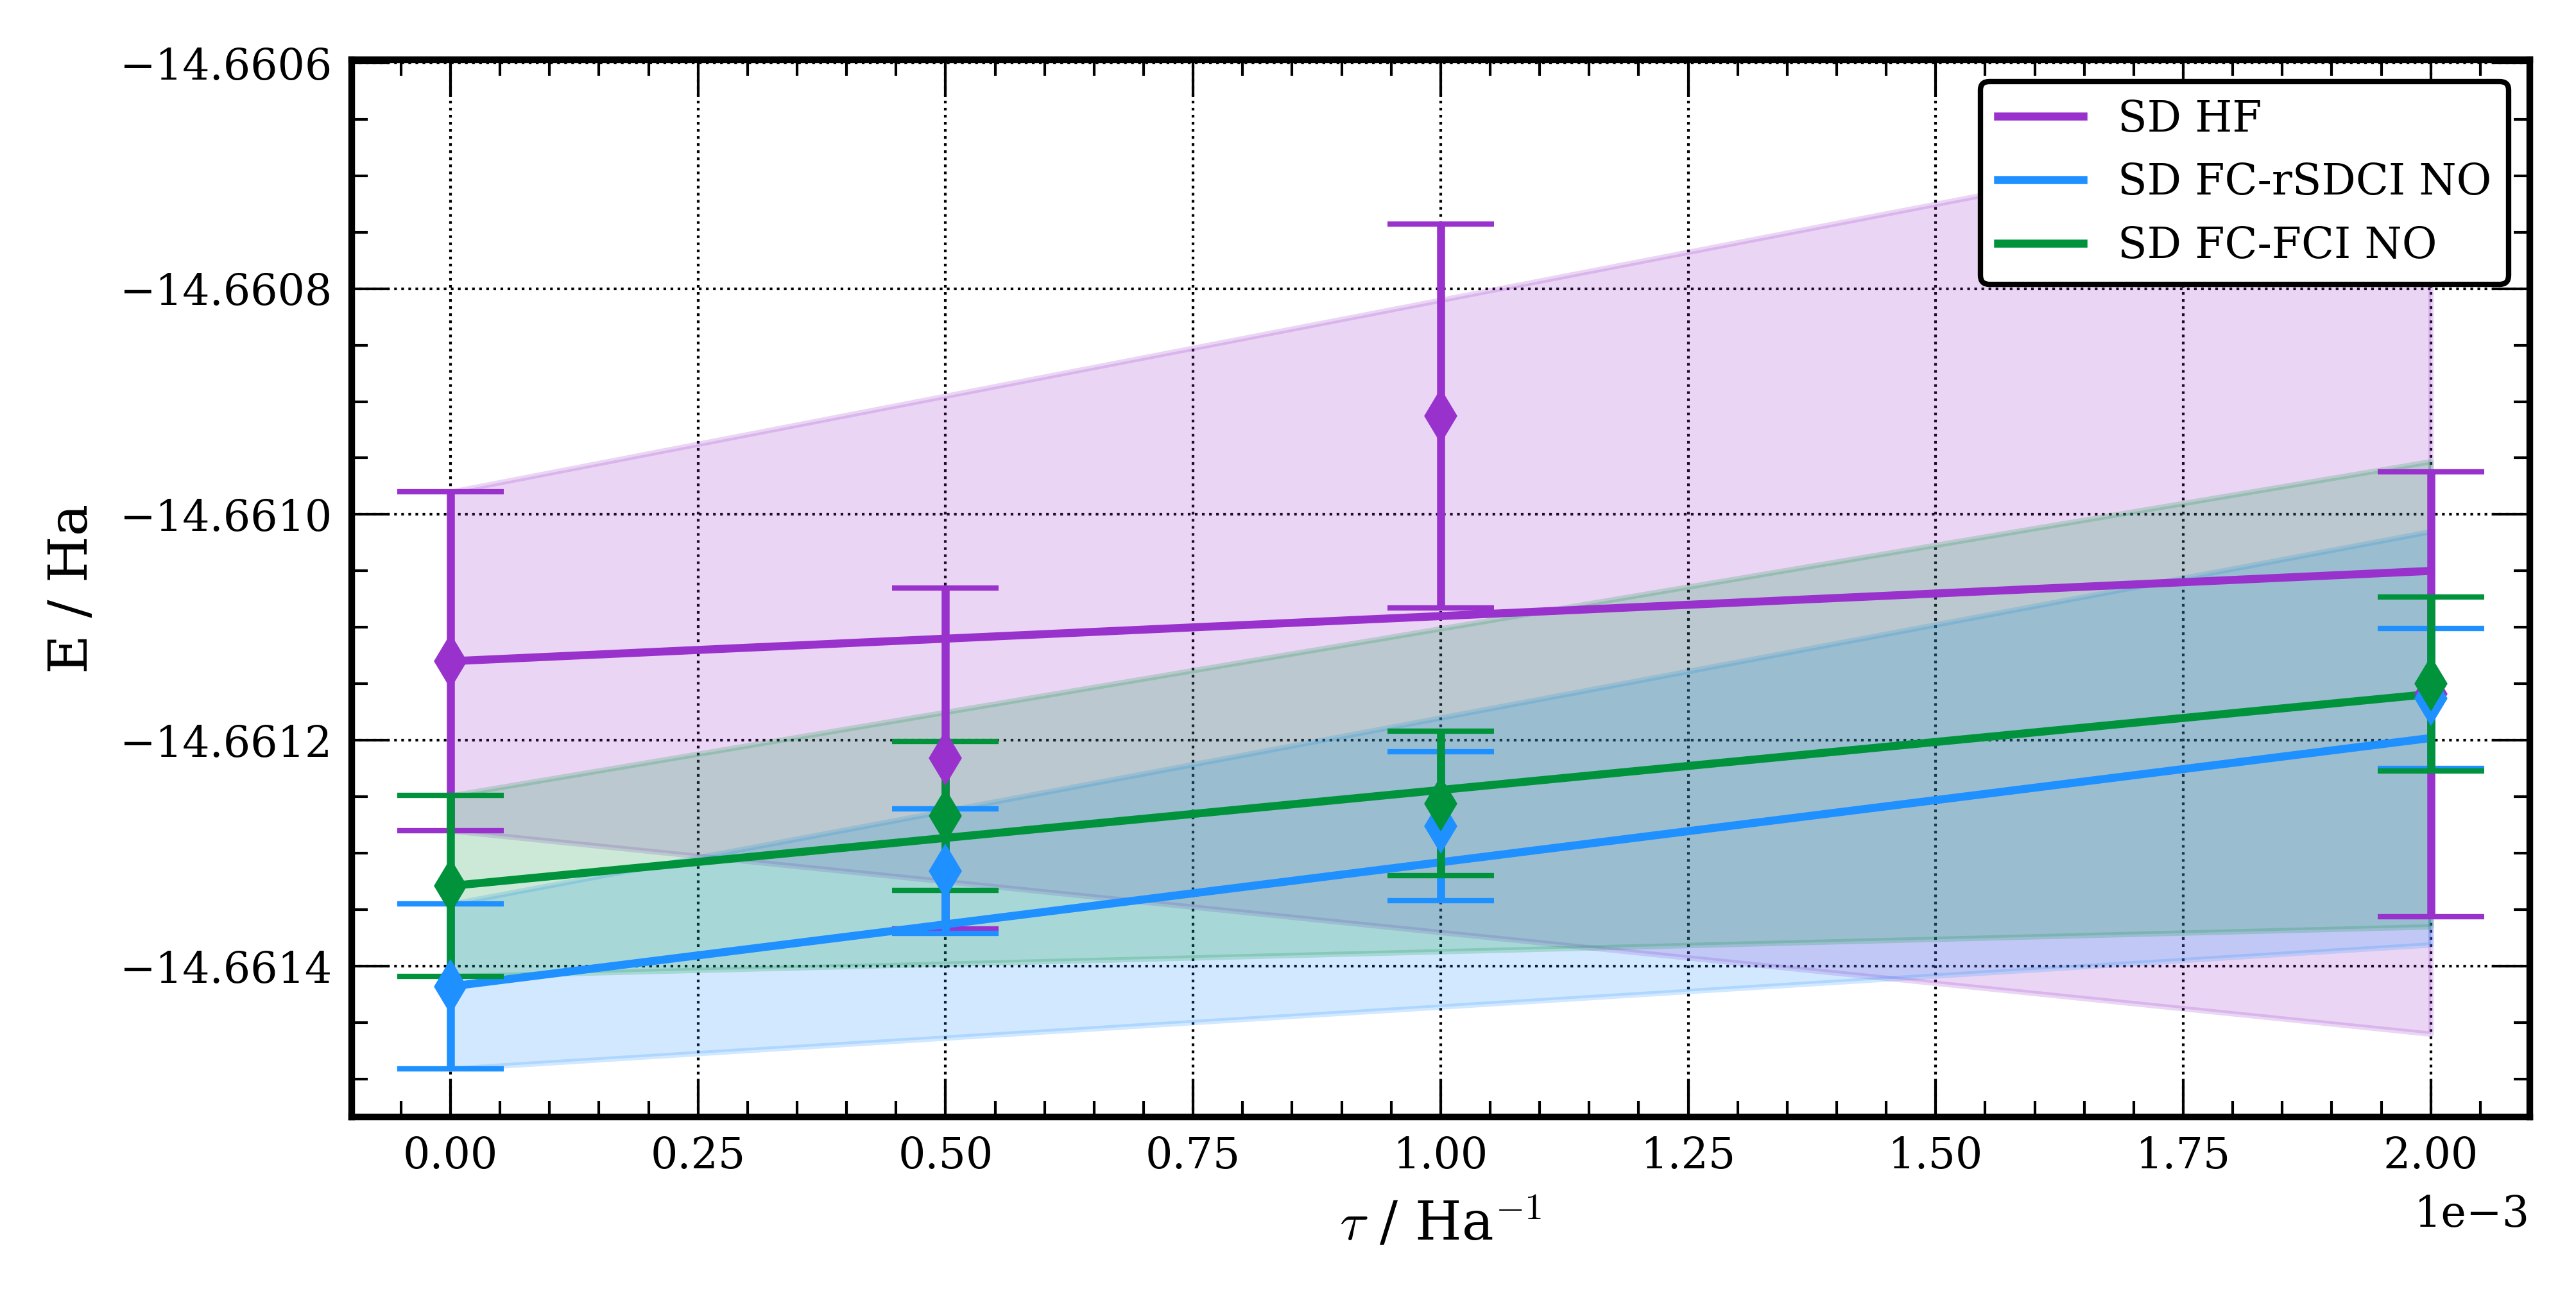
\includegraphics[width=\columnwidth,keepaspectratio]{Images/chapter5/be_extrap_singdet.png}
\end{figure}

%In our results, the nodal surface used captures the electron-positron correlation extremely well in the multi-Slater determinant expansion.
To elucidate the importance of the nodal surface, we plot the \gls{dmc} energy of the \ce{Be}/\ce{e+} system in figure~\ref{fig:be_md_extrap}.
The energy of the \gls{dmc} calculation with a \gls{hf} trial wave function lies significantly far above the correlated trial wave functions.
Including the dispersion effects with the \gls{rSDCI} multi-determinant trial wave function, improves the \gls{dmc} energy, but clearly a significant change in the nodal surface happens once the $s^2\rightarrow p^2$ excitations are included.
Including those excitations by using the \gls{fci} trial wave function, the \gls{dmc} energy drops into excellent agreement with the \gls{svm} reference.
The results from previous \gls{dmc} studies lie higher in energy are included in the plot for reference.\cite{10.1021/acs.jctc.1c01193, 10.1063/1.1486447}

\begin{figure}
    \caption{\label{fig:be_md_extrap} The DMC energy versus time step for \ce{Be} with a bound positron with a Hartree-Fock single determinant trial wave function, frozen core rSDCI multi-determinant trial wave function, and frozen core FCI multi-determinant trial wave function. The reference energies are from \gls{svm}\cite{10.4208/jams.071510.072110a}, DMC\cite{10.1021/acs.jctc.1c01193}, and DMC\cite{10.1063/1.1486447}.
    }
    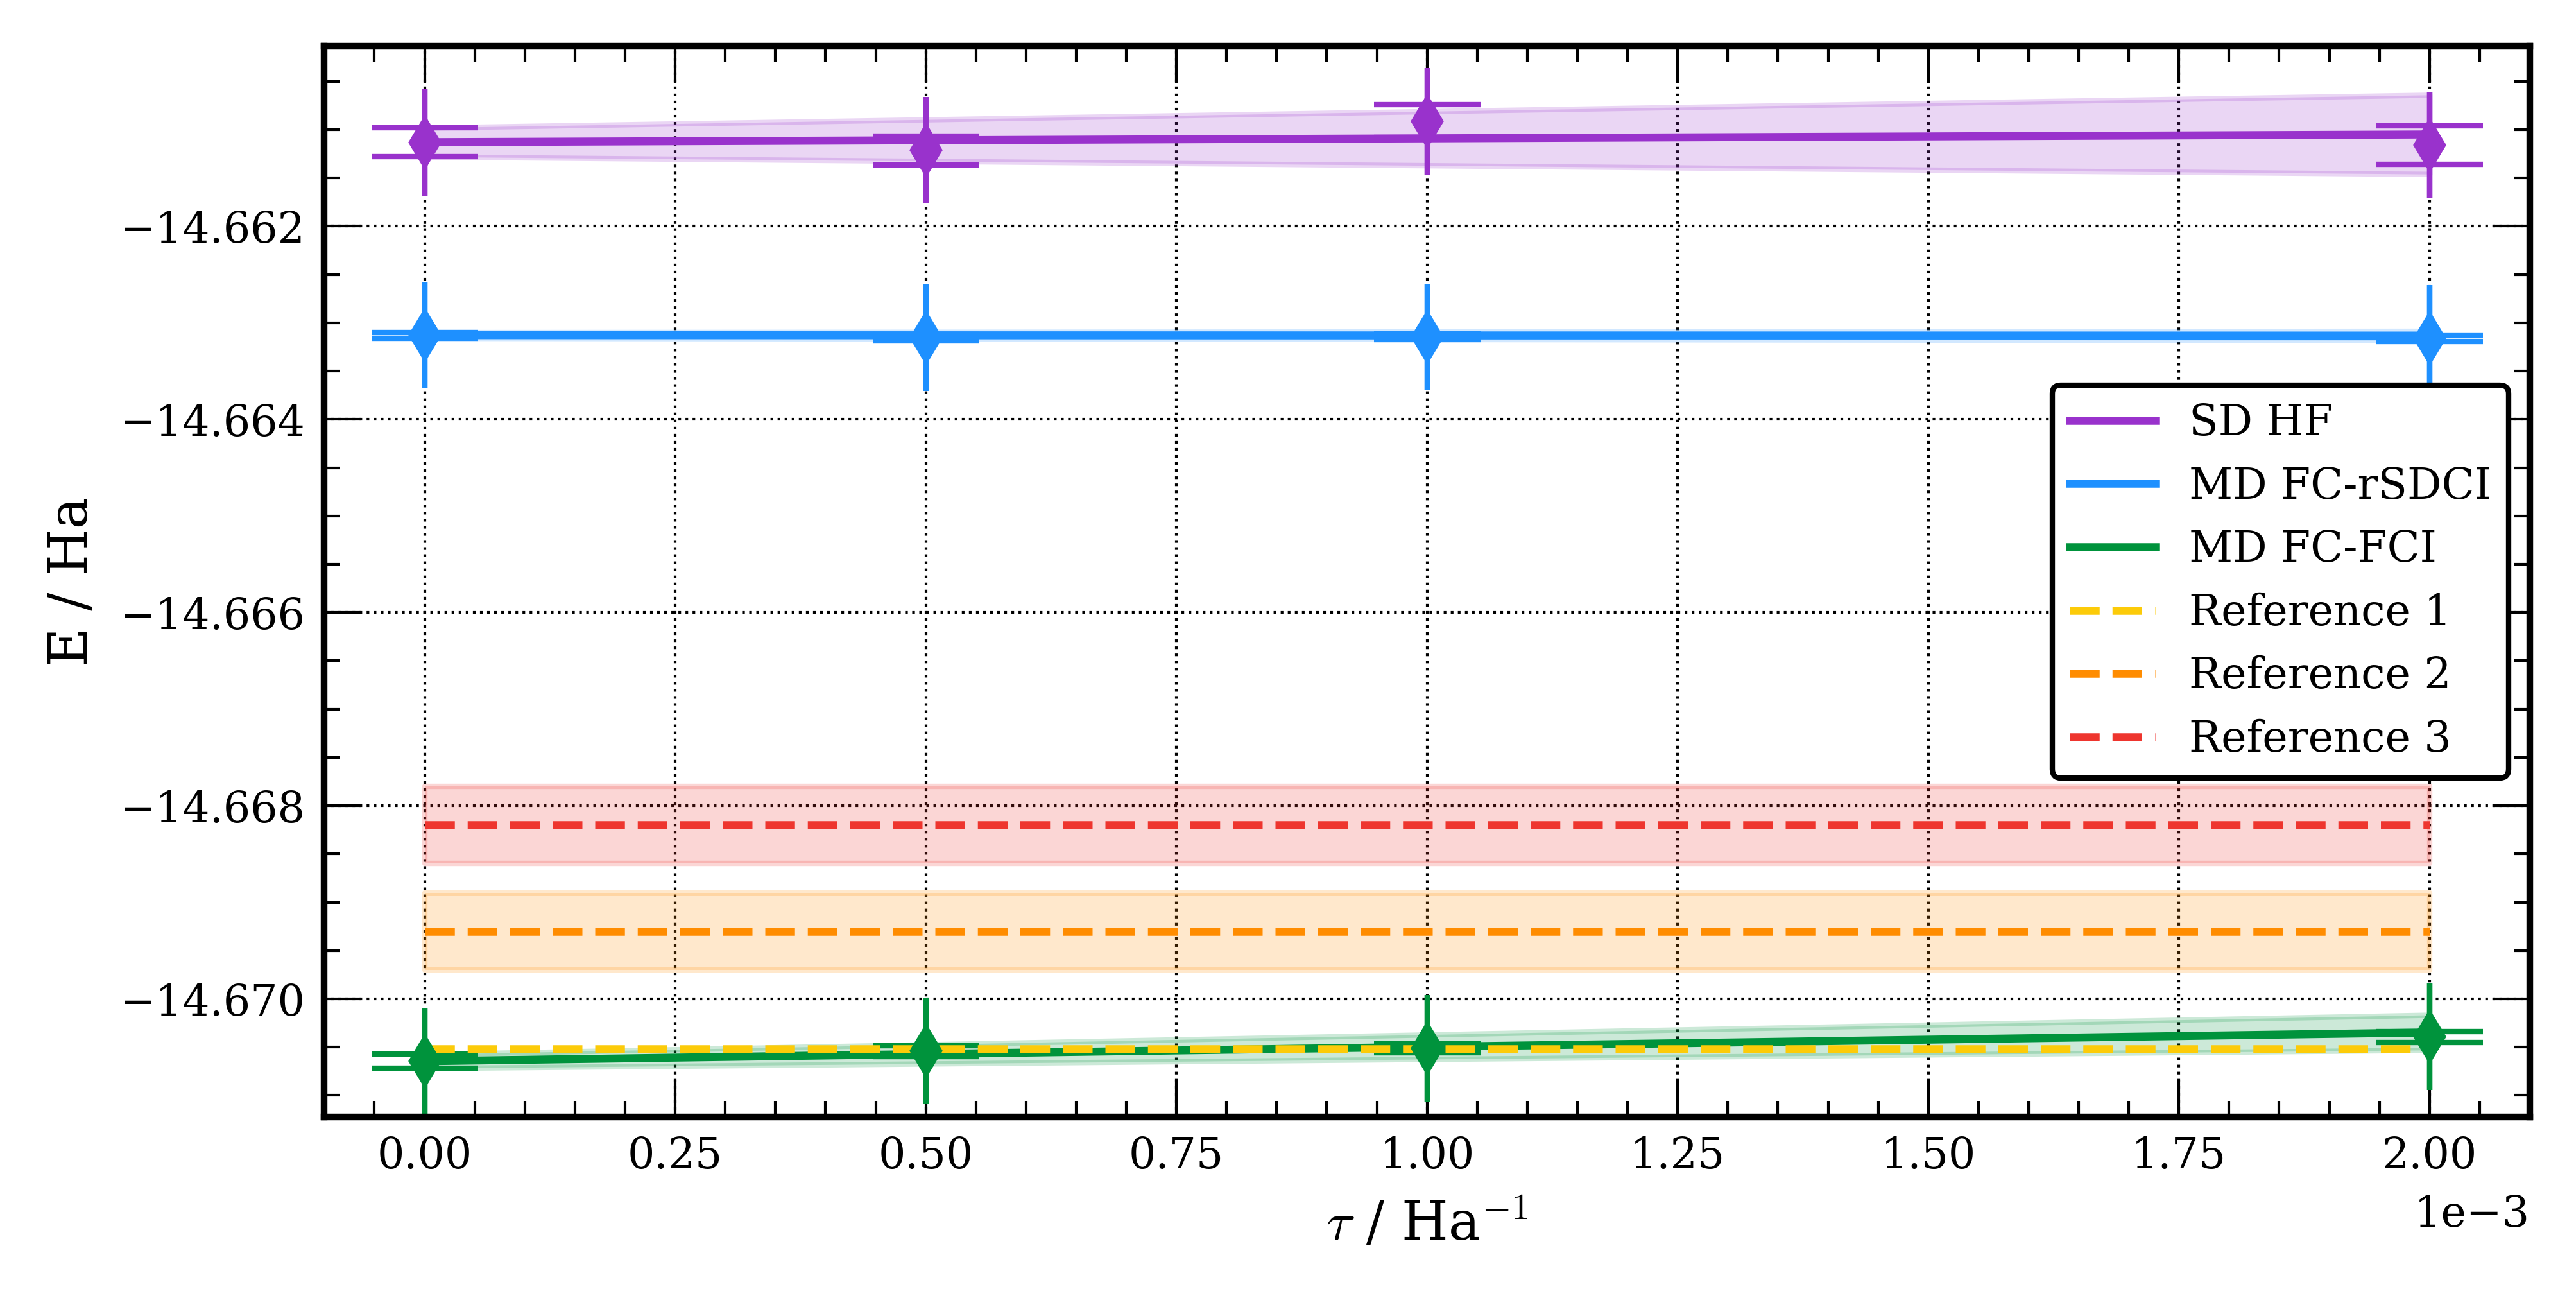
\includegraphics[width=\columnwidth,keepaspectratio]{Images/chapter5/be_extrap_multidet.png}
\end{figure}

We additionally want to comment on a topic with wider implications for the \gls{qmc} field, time step extrapolations for energy differences.
In the literature it has been found that for exitonic binding energies, one can use a very large time step and still resolve the correct energy difference even if the individual energies have an associated time step error.\cite{10.1103/PhysRevB.98.075122}
In figure~\ref{fig:be_e_diff_ts}, we find that for diffuse states such as positron bound states, the time step dependence is still severe.
For a sufficiently small time step however, one is within error bars without extrapolation.
This leads us to recommend caution when resolving energy differences for systems with large relevant length scales, the diffuse positron in this case.

\begin{figure}
    \caption{\label{fig:be_e_diff_ts} DMC positron affinity for \ce{Be} calculated using an rSDCI multi-determinant trial wave function at several time steps sizes. }
    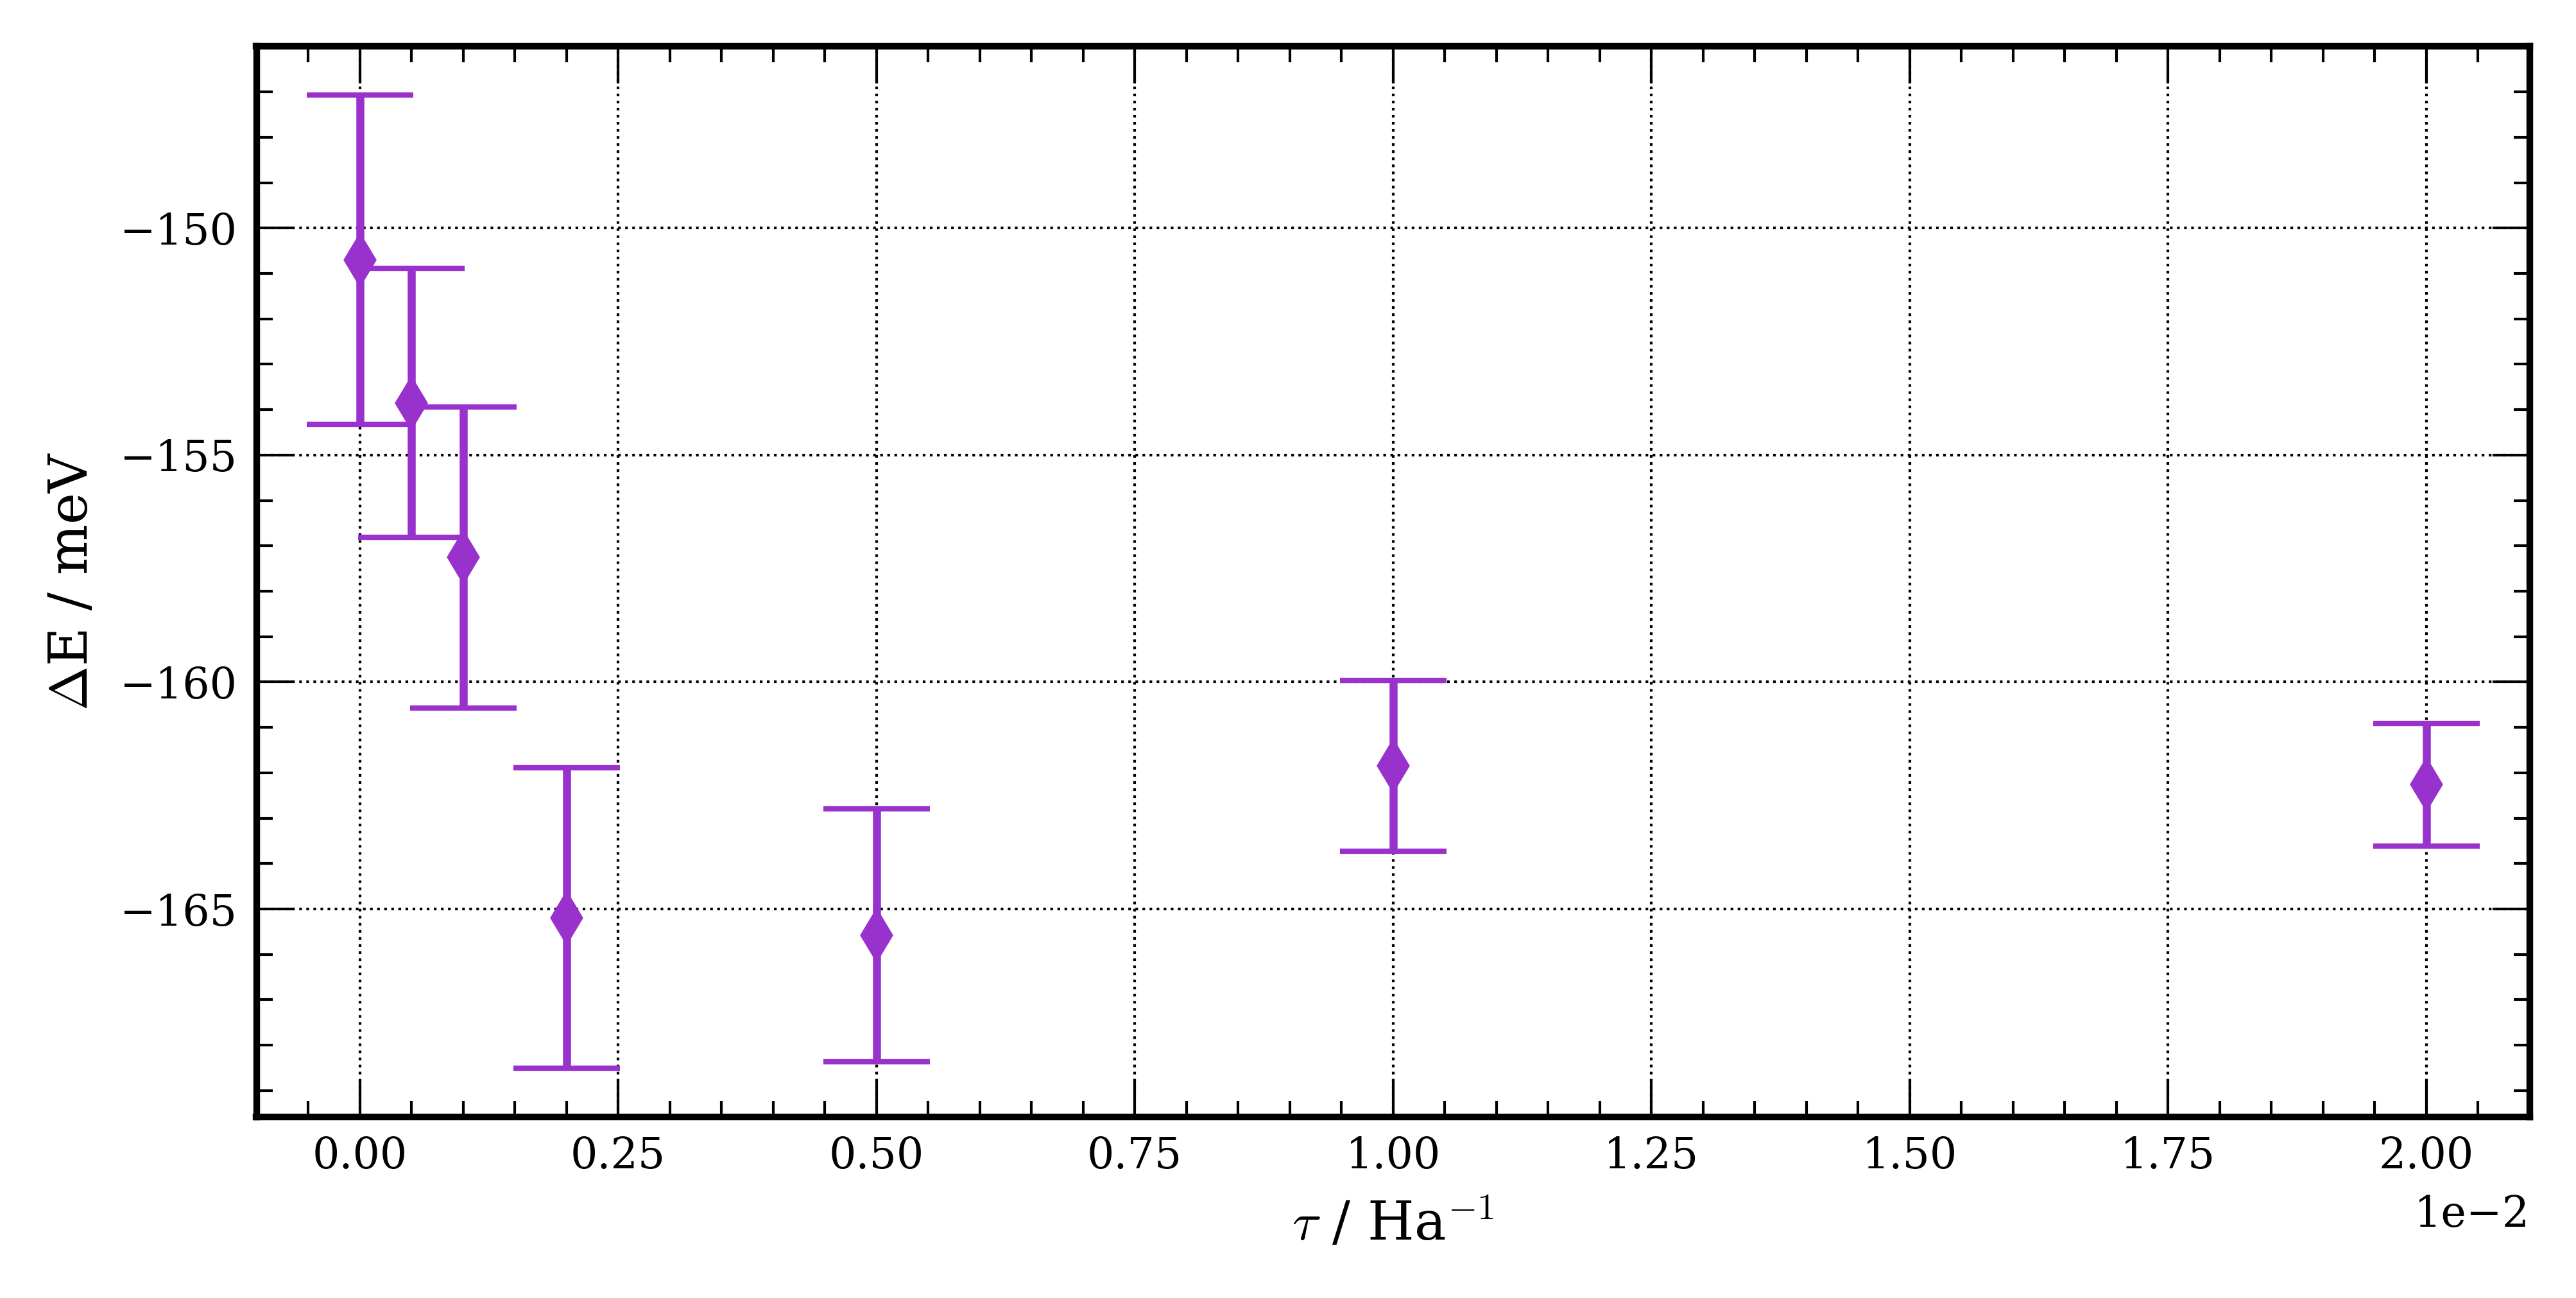
\includegraphics[width=\columnwidth,keepaspectratio]{Images/chapter5/be_rSDCI_multidet.png}
\end{figure}



